\documentclass[slideopt,A4,showboxes,svgnames]{beamer}

%% list of packages here
\usepackage[absolute,showboxes,overlay]{textpos}
\usepackage{booktabs}
\usepackage{mathtools}
\usepackage{amsmath}
\usepackage{amssymb}
\usepackage{pifont}
\usepackage{multicol}
\usepackage{multirow}
\usepackage{array, makecell}
\usepackage{blkarray}
\usepackage{nccmath}
\usepackage[linesnumbered,ruled,vlined]{algorithm2e}
\usepackage[backend=biber, style=authoryear]{biblatex}
\renewcommand*{\nameyeardelim}{\addcomma\addspace}
\addbibresource{../references.bib}

\usepackage{theme/beamerthemeinria}
%

%%%%%%%%%%%%%%%%%%%%%%%%%%%%
% Paper dependent stuff    %
%%%%%%%%%%%%%%%%%%%%%%%%%%%%

\newcommand{\Tau}{\mathcal{T}}
\newcommand{\OurAlgorithm}{\texttt{Constrained-EPC}}
\newcommand{\ux}{\underline{x}}
\newcommand{\ox}{\overline{x}}
\newcommand{\bom}{\bm{\omega}}
\global\long\def\X{\mathbb{X}}%
\global\long\def\U{\mathbb{U}}%


%%%%%%%%%%%%%%%%%%%%%%%%%%%%
% Aesthetics               %
% over-underline, hat, bold%
%%%%%%%%%%%%%%%%%%%%%%%%%%%%

\newcommand{\eps}{\varepsilon}
\newcommand{\vareps}{\varepsilon}
\renewcommand{\epsilon}{\varepsilon}
%\renewcommand{\hat}{\widehat}
\renewcommand{\tilde}{\widetilde}
\renewcommand{\bar}{\overline}

\newcommand*{\MyDef}{\mathrm{\tiny def}}
\newcommand*{\eqdefU}{\ensuremath{\mathop{\overset{\MyDef}{=}}}}% Unscaled version
% \newcommand*{\eqdef}{\mathop{\overset{\MyDef}{\resizebox{\widthof{\eqdefU}}{\heightof{=}}{=}}}}
\newcommand{\eqdef}{\stackrel{def}{=}}


\def\:#1{\protect \ifmmode {\mathbf{#1}} \else {\textbf{#1}} \fi}
\newcommand{\CommaBin}{\mathbin{\raisebox{0.5ex}{,}}}

\newcommand{\wt}[1]{\widetilde{#1}}
\newcommand{\wh}[1]{\widehat{#1}}
\newcommand{\wo}[1]{\overline{#1}}
\newcommand{\wb}[1]{\overline{#1}}

% bf and bm missing due to conflict!!
\newcommand{\bsym}[1]{\mathbf{#1}}
\newcommand{\bzero}{\mathbf{0}}
\newcommand{\ba}{\mathbf{a}}
\newcommand{\bb}{\mathbf{b}}
\newcommand{\bc}{\mathbf{c}}
\newcommand{\bd}{\mathbf{d}}
\newcommand{\be}{\mathbf{e}}
\newcommand{\bg}{\mathbf{g}}
\newcommand{\bh}{\mathbf{h}}
\newcommand{\bi}{\mathbf{i}}
\newcommand{\bj}{\mathbf{j}}
\newcommand{\bk}{\mathbf{k}}
\newcommand{\bl}{\mathbf{l}}
\newcommand{\bn}{\mathbf{n}}
\newcommand{\bo}{\mathbf{o}}
\newcommand{\bp}{\mathbf{p}}
\newcommand{\bq}{\mathbf{q}}
\newcommand{\br}{\mathbf{r}}
\newcommand{\bs}{\mathbf{s}}
\newcommand{\bt}{\mathbf{t}}
\newcommand{\bu}{\mathbf{u}}
\newcommand{\bv}{\mathbf{v}}
\newcommand{\bw}{\mathbf{w}}
\newcommand{\bx}{\mathbf{x}}
\newcommand{\by}{\mathbf{y}}
\newcommand{\bz}{\mathbf{z}}

\newcommand{\bA}{\mathbf{A}}
\newcommand{\bB}{\mathbf{B}}
\newcommand{\bC}{\mathbf{C}}
\newcommand{\bD}{\mathbf{D}}
\newcommand{\bE}{\mathbf{E}}
\newcommand{\bF}{\mathbf{F}}
\newcommand{\bG}{\mathbf{G}}
\newcommand{\bH}{\mathbf{H}}
\newcommand{\bI}{\mathbf{I}}
\newcommand{\bJ}{\mathbf{J}}
\newcommand{\bK}{\mathbf{K}}
\newcommand{\bL}{\mathbf{L}}
\newcommand{\bM}{\mathbf{M}}
\newcommand{\bN}{\mathbf{N}}
\newcommand{\bO}{\mathbf{O}}
\newcommand{\bP}{\mathbf{P}}
\newcommand{\bQ}{\mathbf{Q}}
\newcommand{\bR}{\mathbf{R}}
\newcommand{\bS}{\mathbf{S}}
\newcommand{\bT}{\mathbf{T}}
\newcommand{\bU}{\mathbf{U}}
\newcommand{\bV}{\mathbf{V}}
\newcommand{\bW}{\mathbf{W}}
\newcommand{\bX}{\mathbf{X}}
\newcommand{\bY}{\mathbf{Y}}
\newcommand{\bZ}{\mathbf{Z}}

% calligraphic
\newcommand{\cf}{\mathcal{f}}
\newcommand{\cA}{\mathcal{A}}
\newcommand{\cB}{\mathcal{B}}
\newcommand{\cC}{\mathcal{C}}
\newcommand{\cD}{\mathcal{D}}
\newcommand{\cE}{\mathcal{E}}
\newcommand{\cF}{\mathcal{F}}
\newcommand{\cG}{\mathcal{G}}
\newcommand{\cH}{\mathcal{H}}
\newcommand{\cI}{\mathcal{I}}
\newcommand{\cJ}{\mathcal{J}}
\newcommand{\cK}{\mathcal{K}}
\newcommand{\cL}{\mathcal{L}}
\newcommand{\cM}{\mathcal{M}}
\newcommand{\cN}{\mathcal{N}}
\newcommand{\cO}{\mathcal{O}}
\newcommand{\cP}{\mathcal{P}}
\newcommand{\cQ}{\mathcal{Q}}
\newcommand{\cR}{\mathcal{R}}
\newcommand{\cS}{\mathcal{S}}
\newcommand{\cT}{\mathcal{T}}
\newcommand{\cU}{\mathcal{U}}
\newcommand{\cV}{\mathcal{V}}
\newcommand{\cW}{\mathcal{W}}
\newcommand{\cX}{\mathcal{X}}
\newcommand{\cY}{\mathcal{Y}}
\newcommand{\cZ}{\mathcal{Z}}

%%%%%%%%%%%%%%%%%%%%%%%%%%%%
% Math jargon              %
%%%%%%%%%%%%%%%%%%%%%%%%%%%%
\newcommand{\wrt}{w.r.t.\xspace}
\newcommand{\defeq}{\stackrel{\mathclap{\normalfont\mbox{\tiny def}}}{=}}
\newcommand{\maxund}[1]{\max\limits_{#1}}
\newcommand{\supund}[1]{\text{sup}\limits_{#1}}
\newcommand{\minund}[1]{\min\limits_{#1}}
\renewcommand{\epsilon}{\varepsilon}
\newcommand{\bigotime}{\mathcal{O}}
\newcommand{\dd}{\mathrm{d}}

\DeclareMathOperator*{\argmin}{arg\,min} 
\DeclareMathOperator*{\argmax}{arg\,max} 
\DeclareMathOperator*{\cupdot}{\mathbin{\mathaccent\cdot\cup}}

%%%%%%%%%%%%%%%%%%%%%%%%%%%%
% Matrix operators         %
%%%%%%%%%%%%%%%%%%%%%%%%%%%%
\newcommand{\transpose}{^\mathsf{\scriptscriptstyle T}}
%\newcommand{\transp}{\mathsf{\scriptscriptstyle T}}
\newcommand{\transp}{\top}
\DeclareMathOperator{\Tr}{Tr}
\DeclarePairedDelimiterX{\inp}[2]{\langle}{\rangle}{#1, #2}

%%%%%%%%%%%%%%%%%%%%%%%%%%%%
% Statistic operators      %
%%%%%%%%%%%%%%%%%%%%%%%%%%%%
\newcommand{\probability}[1]{\mathbb{P}\left(#1\right)}
\newcommand{\probdist}{Pr}
\DeclareMathOperator*{\expectedvalue}{\mathbb{E}}
\DeclareMathOperator*{\variance}{\text{Var}}
\newcommand{\expectedvalueover}[1]{\expectedvalue\limits_{#1}}
\newcommand{\condbar}{\;\middle|\;}
\newcommand{\gaussdistr}{\mathcal{N}}
\newcommand{\uniformdistr}{\mathcal{U}}
\newcommand{\bernoullidist}{\mathcal{B}}

%%%%%%%%%%%%%%%%%%%%%%%%%%%%
% Algebraic Sets           %
%%%%%%%%%%%%%%%%%%%%%%%%%%%%
\newcommand{\Real}{\mathbb{R}}
\newcommand{\Natural}{\mathbb{N}}
\newcommand{\statespace}{\mathcal{X}}
\newcommand{\funcspace}{\mathcal{F}}
\newcommand{\dynaspace}{\mathcal{T}}


%\newtheorem{theorem}{Theorem}
%\newtheorem{definition}{Definition}
%\newtheorem{corollary}{Corollary}
%\newtheorem{lemma}{Lemma}
\providecommand*\lemmaautorefname{Lemma}
\newtheorem{proposition}{Proposition}
\providecommand*\propositionautorefname{Proposition}
\newtheorem{remark}{Remark}
\newtheorem{property}{Property}
\newtheorem{assumption}{Assumption}
\providecommand*\assumptionautorefname{Assumption}
\newtheorem{conjecture}{Conjecture}
\providecommand*\algorithmautorefname{Algorithm}



%%%%%%%%%%%%%%%%%%%%%%%%%%%%
% Paper dependent stuff    %
%%%%%%%%%%%%%%%%%%%%%%%%%%%%

\newcommand{\Tau}{\mathcal{T}}
\newcommand{\OurAlgorithm}{\texttt{Constrained-EPC}}
\newcommand{\ux}{\underline{x}}
\newcommand{\ox}{\overline{x}}
\newcommand{\bom}{\bm{\omega}}
\global\long\def\X{\mathbb{X}}%
\global\long\def\U{\mathbb{U}}%


%%%%%%%%%%%%%%%%%%%%%%%%%%%%
% Aesthetics               %
% over-underline, hat, bold%
%%%%%%%%%%%%%%%%%%%%%%%%%%%%

\newcommand{\eps}{\varepsilon}
\newcommand{\vareps}{\varepsilon}
\renewcommand{\epsilon}{\varepsilon}
%\renewcommand{\hat}{\widehat}
\renewcommand{\tilde}{\widetilde}
\renewcommand{\bar}{\overline}

\newcommand*{\MyDef}{\mathrm{\tiny def}}
\newcommand*{\eqdefU}{\ensuremath{\mathop{\overset{\MyDef}{=}}}}% Unscaled version
% \newcommand*{\eqdef}{\mathop{\overset{\MyDef}{\resizebox{\widthof{\eqdefU}}{\heightof{=}}{=}}}}
\newcommand{\eqdef}{\stackrel{def}{=}}


\def\:#1{\protect \ifmmode {\mathbf{#1}} \else {\textbf{#1}} \fi}
\newcommand{\CommaBin}{\mathbin{\raisebox{0.5ex}{,}}}

\newcommand{\wt}[1]{\widetilde{#1}}
\newcommand{\wh}[1]{\widehat{#1}}
\newcommand{\wo}[1]{\overline{#1}}
\newcommand{\wb}[1]{\overline{#1}}

% bf and bm missing due to conflict!!
\newcommand{\bsym}[1]{\mathbf{#1}}
\newcommand{\bzero}{\mathbf{0}}
\newcommand{\ba}{\mathbf{a}}
\newcommand{\bb}{\mathbf{b}}
\newcommand{\bc}{\mathbf{c}}
\newcommand{\bd}{\mathbf{d}}
\newcommand{\be}{\mathbf{e}}
\newcommand{\bg}{\mathbf{g}}
\newcommand{\bh}{\mathbf{h}}
\newcommand{\bi}{\mathbf{i}}
\newcommand{\bj}{\mathbf{j}}
\newcommand{\bk}{\mathbf{k}}
\newcommand{\bl}{\mathbf{l}}
\newcommand{\bn}{\mathbf{n}}
\newcommand{\bo}{\mathbf{o}}
\newcommand{\bp}{\mathbf{p}}
\newcommand{\bq}{\mathbf{q}}
\newcommand{\br}{\mathbf{r}}
\newcommand{\bs}{\mathbf{s}}
\newcommand{\bt}{\mathbf{t}}
\newcommand{\bu}{\mathbf{u}}
\newcommand{\bv}{\mathbf{v}}
\newcommand{\bw}{\mathbf{w}}
\newcommand{\bx}{\mathbf{x}}
\newcommand{\by}{\mathbf{y}}
\newcommand{\bz}{\mathbf{z}}

\newcommand{\bA}{\mathbf{A}}
\newcommand{\bB}{\mathbf{B}}
\newcommand{\bC}{\mathbf{C}}
\newcommand{\bD}{\mathbf{D}}
\newcommand{\bE}{\mathbf{E}}
\newcommand{\bF}{\mathbf{F}}
\newcommand{\bG}{\mathbf{G}}
\newcommand{\bH}{\mathbf{H}}
\newcommand{\bI}{\mathbf{I}}
\newcommand{\bJ}{\mathbf{J}}
\newcommand{\bK}{\mathbf{K}}
\newcommand{\bL}{\mathbf{L}}
\newcommand{\bM}{\mathbf{M}}
\newcommand{\bN}{\mathbf{N}}
\newcommand{\bO}{\mathbf{O}}
\newcommand{\bP}{\mathbf{P}}
\newcommand{\bQ}{\mathbf{Q}}
\newcommand{\bR}{\mathbf{R}}
\newcommand{\bS}{\mathbf{S}}
\newcommand{\bT}{\mathbf{T}}
\newcommand{\bU}{\mathbf{U}}
\newcommand{\bV}{\mathbf{V}}
\newcommand{\bW}{\mathbf{W}}
\newcommand{\bX}{\mathbf{X}}
\newcommand{\bY}{\mathbf{Y}}
\newcommand{\bZ}{\mathbf{Z}}

% calligraphic
\newcommand{\cf}{\mathcal{f}}
\newcommand{\cA}{\mathcal{A}}
\newcommand{\cB}{\mathcal{B}}
\newcommand{\cC}{\mathcal{C}}
\newcommand{\cD}{\mathcal{D}}
\newcommand{\cE}{\mathcal{E}}
\newcommand{\cF}{\mathcal{F}}
\newcommand{\cG}{\mathcal{G}}
\newcommand{\cH}{\mathcal{H}}
\newcommand{\cI}{\mathcal{I}}
\newcommand{\cJ}{\mathcal{J}}
\newcommand{\cK}{\mathcal{K}}
\newcommand{\cL}{\mathcal{L}}
\newcommand{\cM}{\mathcal{M}}
\newcommand{\cN}{\mathcal{N}}
\newcommand{\cO}{\mathcal{O}}
\newcommand{\cP}{\mathcal{P}}
\newcommand{\cQ}{\mathcal{Q}}
\newcommand{\cR}{\mathcal{R}}
\newcommand{\cS}{\mathcal{S}}
\newcommand{\cT}{\mathcal{T}}
\newcommand{\cU}{\mathcal{U}}
\newcommand{\cV}{\mathcal{V}}
\newcommand{\cW}{\mathcal{W}}
\newcommand{\cX}{\mathcal{X}}
\newcommand{\cY}{\mathcal{Y}}
\newcommand{\cZ}{\mathcal{Z}}

%%%%%%%%%%%%%%%%%%%%%%%%%%%%
% Math jargon              %
%%%%%%%%%%%%%%%%%%%%%%%%%%%%
\newcommand{\wrt}{w.r.t.\xspace}
\newcommand{\defeq}{\stackrel{\mathclap{\normalfont\mbox{\tiny def}}}{=}}
\newcommand{\maxund}[1]{\max\limits_{#1}}
\newcommand{\supund}[1]{\text{sup}\limits_{#1}}
\newcommand{\minund}[1]{\min\limits_{#1}}
\renewcommand{\epsilon}{\varepsilon}
\newcommand{\bigotime}{\mathcal{O}}
\newcommand{\dd}{\mathrm{d}}

\DeclareMathOperator*{\argmin}{arg\,min} 
\DeclareMathOperator*{\argmax}{arg\,max} 
\DeclareMathOperator*{\cupdot}{\mathbin{\mathaccent\cdot\cup}}

%%%%%%%%%%%%%%%%%%%%%%%%%%%%
% Matrix operators         %
%%%%%%%%%%%%%%%%%%%%%%%%%%%%
\newcommand{\transpose}{^\mathsf{\scriptscriptstyle T}}
%\newcommand{\transp}{\mathsf{\scriptscriptstyle T}}
\newcommand{\transp}{\top}
\DeclareMathOperator{\Tr}{Tr}
\DeclarePairedDelimiterX{\inp}[2]{\langle}{\rangle}{#1, #2}

%%%%%%%%%%%%%%%%%%%%%%%%%%%%
% Statistic operators      %
%%%%%%%%%%%%%%%%%%%%%%%%%%%%
\newcommand{\probability}[1]{\mathbb{P}\left(#1\right)}
\newcommand{\probdist}{Pr}
\DeclareMathOperator*{\expectedvalue}{\mathbb{E}}
\DeclareMathOperator*{\variance}{\text{Var}}
\newcommand{\expectedvalueover}[1]{\expectedvalue\limits_{#1}}
\newcommand{\condbar}{\;\middle|\;}
\newcommand{\gaussdistr}{\mathcal{N}}
\newcommand{\uniformdistr}{\mathcal{U}}
\newcommand{\bernoullidist}{\mathcal{B}}

%%%%%%%%%%%%%%%%%%%%%%%%%%%%
% Algebraic Sets           %
%%%%%%%%%%%%%%%%%%%%%%%%%%%%
\newcommand{\Real}{\mathbb{R}}
\newcommand{\Natural}{\mathbb{N}}
\newcommand{\statespace}{\mathcal{X}}
\newcommand{\funcspace}{\mathcal{F}}
\newcommand{\dynaspace}{\mathcal{T}}


%\newtheorem{theorem}{Theorem}
%\newtheorem{definition}{Definition}
%\newtheorem{corollary}{Corollary}
%\newtheorem{lemma}{Lemma}
\providecommand*\lemmaautorefname{Lemma}
\newtheorem{proposition}{Proposition}
\providecommand*\propositionautorefname{Proposition}
\newtheorem{remark}{Remark}
\newtheorem{property}{Property}
\newtheorem{assumption}{Assumption}
\providecommand*\assumptionautorefname{Assumption}
\newtheorem{conjecture}{Conjecture}
\providecommand*\algorithmautorefname{Algorithm}


% Colors for slides
\definecolor{rouge1}{RGB}{226,0,38}  % red P
\definecolor{orange1}{RGB}{243,154,38}  % orange P
\definecolor{jaune}{RGB}{254,205,27}  % jaune P
\definecolor{blanc}{RGB}{255,255,255} % blanc P

\definecolor{rouge2}{RGB}{230,68,57}  % red S
\definecolor{orange2}{RGB}{236,117,40}  % orange S
\definecolor{taupe}{RGB}{134,113,127} % taupe S
\definecolor{gris}{RGB}{91,94,111} % gris S
\definecolor{bleu1}{RGB}{38,109,131} % bleu S
\definecolor{bleu2}{RGB}{28,50,114} % bleu S
\definecolor{vert1}{RGB}{133,146,66} % vert S
\definecolor{vert3}{RGB}{20,200,66} % vert S
\definecolor{vert2}{RGB}{157,193,7} % vert S
\definecolor{vertsolarized}{RGB}{211,233,219} % vert S
\definecolor{darkyellow}{RGB}{233,165,0}  % orange S
\definecolor{lightgray}{rgb}{0.9,0.9,0.9}
\definecolor{darkgray}{rgb}{0.6,0.6,0.6}

\newcommand{\incarrow}{{
\includegraphics[height=0.7\baselineskip]{./theme/img/arrow_list}}}


% Highlights for slides
\newcommand{\rcol}[1]{\textcolor{red}{\textit{#1}}}
%\newcommand{\eqrcol}[1]{\textcolor{red}{#1}}
%\newcommand{\eqrcolb}[1]{\textcolor{red}{\boldsymbol{#1}}}
\newcommand{\gcol}[1]{\textcolor{vert3}{\textit{#1}}}
%\newcommand{\eqgcol}[1]{\textcolor{vert3}{#1}}
%\newcommand{\eqgcolb}[1]{\textcolor{vert3}{\boldsymbol{#1}}}
\newcommand{\blcol}[1]{\textcolor{blue}{\textit{#1}}}
%\newcommand{\eqbcol}[1]{\textcolor{blue}{#1}}
%\newcommand{\eqbcolb}[1]{\textcolor{blue}{\boldsymbol{#1}}}
\newcommand{\ycol}[1]{\textcolor{darkyellow}{\textit{#1}}}
\newcommand{\eqycol}[1]{\textcolor{darkyellow}{#1}}

\newcommand{\rcolbm}[1]{$\textcolor{red}{\boldsymbol{#1}}$}
\newcommand{\rcolb}[1]{\textcolor{red}{\textit{\textbf{#1}}}}
\newcommand{\gcolb}[1]{\textcolor{vert3}{\textit{\textbf{#1}}}}
\newcommand{\bcolb}[1]{\textcolor{blue}{\textit{\textbf{#1}}}}
\newcommand{\ycolb}[1]{\textcolor{darkyellow}{\textit{\textbf{#1}}}}

% Colored boxes
\newcounter{ColoredBoxesCounter}
\newcommand{\highlightnew}[3][(0.0,-0.1)(-0.0,0.3)]{
\hfsetfillcolor{#2!20}
\hfsetbordercolor{#2!80}
\tikzmarkin{\theColoredBoxesCounter}#1
#3
\tikzmarkend{\theColoredBoxesCounter}
\stepcounter{ColoredBoxesCounter}
}

\newcommand{\highlight}[2][yellow]{\mathchoice%
{\colorbox{#1}{$\displaystyle#2$}}%
{\colorbox{#1}{$\textstyle#2$}}%
{\colorbox{#1}{$\scriptstyle#2$}}%
{\colorbox{#1}{$\scriptscriptstyle#2$}}}%

\newcommand{\eqrcol}[1]{\highlight[red!20]{#1}}
\newcommand{\eqrcolb}[1]{\highlight[red!20]{\boldsymbol{#1}}}
\newcommand{\eqgcol}[1]{\highlight[vert3!20]{#1}}
\newcommand{\eqgcolb}[1]{\highlight[vert3!20]{\boldsymbol{#1}}}
\newcommand{\eqbcol}[1]{\highlight[blue!20]{#1}}
\newcommand{\eqbcolb}[1]{\highlight[blue!20]{\boldsymbol{#1}}}

\colorlet{redp}{red!20} % vert S
\colorlet{greenp}{vert3!20} % vert S
\colorlet{bluep}{blue!20} % vert S
\colorlet{yellowp}{yellow!20} % vert S

\usepackage{soul}
\renewcommand{\hl}[3][\fboxsep1pt]{{#1\colorbox{#2}{#3}}}%

\newcommand{\hlr}[1]{\hl{redp}{#1}}
\newcommand{\hlg}[1]{\hl{greenp}{#1}}
\newcommand{\hlb}[1]{\hl{bluep}{#1}}
\newcommand{\hly}[1]{\hl{yellowp}{#1}}

\newcommand{\hler}[1]{\hl[\fboxsep0pt]{redp}{$\displaystyle {#1}$}}
\newcommand{\hleg}[1]{\hl[\fboxsep0pt]{greenp}{$\displaystyle {#1}$}}
\newcommand{\hleb}[1]{\hl[\fboxsep0pt]{bluep}{$\displaystyle {#1}$}}

\newcommand{\hlbr}[1]{\hl[\fboxsep0pt]{redp}{$\displaystyle \mathbf{#1}$}}
\newcommand{\hlbg}[1]{\hl[\fboxsep0pt]{greenp}{$\displaystyle \mathbf{#1}$}}
\newcommand{\hlbb}[1]{\hl[\fboxsep0pt]{bluep}{$\displaystyle \mathbf{#1}$}}

\newcommand{\vph}{\vphantom{A_A^A}}

% Box for algorithms
\newlength{\minipagewidth}
\newlength{\minipagewidthx}
\setlength{\minipagewidth}{\columnwidth}
\setlength{\minipagewidthx}{\columnwidth}
\setlength{\fboxsep}{0.1mm}
\addtolength{\minipagewidth}{-\fboxrule}
\addtolength{\minipagewidth}{-\fboxrule}
\addtolength{\minipagewidth}{-\fboxsep}
\addtolength{\minipagewidth}{-\fboxsep}
\addtolength{\minipagewidthx}{+\fboxsep}
\newcommand{\bookbox}[1]{\small
\par\medskip\noindent
\framebox[\columnwidth]{
\begin{minipage}{\minipagewidth} {#1} \end{minipage} } \par\medskip }

\newcommand{\bookboxx}[1]{
\par\medskip\noindent
\framebox[\columnwidth]{
\begin{minipage}[t]{0.98\columnwidth} {\par\smallskip#1\par\smallskip} \end{minipage} } \par\medskip }


\usepackage{array}
\newcolumntype{L}[1]{>{\raggedright\let\newline\\\arraybackslash\hspace{-3.1cm}}m{#1}}
\newcolumntype{C}[1]{>{\centering\let\newline\\\arraybackslash\hspace{135pt}}m{#1}}
\newcolumntype{R}[1]{>{\raggedleft\let\newline\\\arraybackslash\hspace{-10pt}}m{#1}}

\newenvironment{myfont}{\fontfamily{kurier}\selectfont}{\par}
\newenvironment{myfont2}{\fontfamily{epigrafica}\selectfont}{\par}

% Border color of content boxes
\definecolor{bordercol}{RGB}{0,0,0}  %black
% Background color for the header in the content boxes (left side)
\definecolor{headercol1}{RGB}{200,0,0}        %red:RGB {200,0,0} 
% Background color for the header in the content boxes (right side) 
\definecolor{headercol2}{rgb}{1.0,0.49,0.0}        %orange:rgb {1.0,0.49,0.0}
% Text color for the header text in the content boxes
\definecolor{headerfontcol}{rgb}{1,1,1}  %white
% Background color for the content in the boxes
\definecolor{boxcolor}{rgb}{1,1,1} 

\definecolor{lightblue}{rgb}{0.145,0.6666,1}

\newsavebox\CBox
\newcommand\hcancel[2][0.5pt]{%
  \ifmmode\sbox\CBox{$#2$}\else\sbox\CBox{#2}\fi%
  \makebox[0pt][l]{\usebox\CBox}%  
  \rule[0.3\ht\CBox-#1/2]{\wd\CBox}{#1}}


\title[Robust-Adaptive Control]{Robust-Adaptive\\Interval Predictive Control\\ for Linear Uncertain Systems}
\subtitle{Sous-titre}
\date[date]{date}
\author[Edouard Leurent]{\textbf{Edouard Leurent}\inst{1,2},\\
	Odalric-Ambrym Maillard\inst{1},\\
	Denis Efimov\inst{1}}
\institute{
	\inst{1} Univ. Lille, Inria, CNRS, \\ ~Centrale Lille, UMR 9189 – CRIStAL,\\
	\inst{2} Renault Group}

\begin{document}

\begin{frame}
    \titlepage
\end{frame}

\begin{frame}{Motivation}


Real-world systems face a severe model uncertainty
under strict state and control constraints, whose maintaining is critical and related with the system safety

\end{frame}

\begin{frame}{Setting}
\begin{exampleblock}{Objective}
\begin{itemize}
	\item Stabilization of a linear system \useshortskip
	\begin{align*}
	{\dot{x}(t)} &= \textcolor<4>{orange}{A(\theta)}{x(t)} + B u(t) + \textcolor<2-4>{normalBlockTitleTextColor}{\omega(t)},
	\end{align*}
	\item Constraints on state $x\in\X$, control $u\in\U$.
\end{itemize}
\end{exampleblock}
\pause
\begin{alertblock}{Subject to uncertainty}
	\begin{itemize}[<+->]
		\item Bounded disturbance ${\red \underline\omega(t) \leq \omega(t) \leq \overline\omega(t)}$;
		\item Bounded measurement noise ${\red \underline\eta(t) \leq \eta(t) \leq \overline\eta(t)}$,
		\useshortskip
		\begin{equation*} y(t) = \begin{bmatrix}x(t) & \dot x(t)\end{bmatrix}^\top + {\red \eta(t)};\end{equation*}
		\item Parametric uncertainty in the state matrix \useshortskip
	\begin{align*}
	{\orange A(\theta)} = A + \sum_{i=1}^d {\orange \theta_i}\phi_i\text{ is unknown.}
	\end{align*}
	\end{itemize}\vspace*{-0.5cm}
\end{alertblock}
\end{frame}

\begin{frame}{Related work}

\begin{alertblock}{Adaptive Model Predictive Control (MPC)}
	See \textit{e.g.} [\cite{Fukushima2007,Adetola2009,Adetola2011,Aswani2013,Vicente2019}]
	\pause
	\begin{enumerate}[<+->]
		\item Estimation algorithm to evaluate the model uncertainty
		\item MPC to enforce constraints during transients
	\end{enumerate}
\end{alertblock}
\pause[\thebeamerpauses]
\begin{exampleblock}{Our work}
	\begin{itemize}
		\item A simple solution using \alert{intervals},
		\item based on a \alert{recent predictor} [\cite{leurent2019interval}]
	\end{itemize}
\end{exampleblock}
\end{frame}

\begin{frame}{Step 1: Model Estimation}
\begin{assumption}[Persistence of Excitation (PE)]
	\label{assu:PE}
	The features $\Phi(t)=[\phi_{1}y_{1}(t)\dots\phi_{d}y_{1}(t)]\in\Real^{p\times d}$ verify
	\[\forall t\geq 0,\;
	\int_{t}^{t+\ell}\Phi^{\top}(s)\Phi(s)ds\ge\vartheta I_{d}.
	\]
\end{assumption}
\pause
Define \begin{equation*}
\hat{\theta}(t)=
\left(\int_{0}^{t}\Phi^{\top}(s)\Phi(s)ds\right)^{-1}\int_{0}^{t}\Phi^{\top}(s)y(s)ds,\, t\geq\ell,
\end{equation*}
\pause
\begin{proposition}[Admissible values $\hat{\Theta}(t)\subseteq\Theta$]
%For all $t\geq\ell$,
%	$
%	|\hat{\theta}(t)-\theta|\leq\Delta\theta(\Vert x\Vert_{\infty})
%	$
	\begin{equation*}
	\theta \in {\orange \hat{\Theta}(t)}=\Theta\bigcap_{\tau\in[\ell,t]}\{\tilde{\theta}\in\Real^{d}:|\hat{\theta}(\tau)-\tilde{\theta}|\leq\Delta\theta(X)\}.\label{eq:set_LS}
	\end{equation*}
\end{proposition}
\end{frame}

\begin{frame}{Step 2: State Prediction}
Given $\orange \hat{\Theta}(t)$, ${\red \underline\omega(s) \leq \omega(s) \leq \overline\omega(s)}$, ${\red \underline\eta(s) \leq \eta(s) \leq \overline\eta(s)}$, we want: 
\begin{equation*}
{\blue \ux(s)}\leq x(s)\leq{\blue \ox(s)},\quad\forall s\geq t.
\end{equation*}

\begin{center}
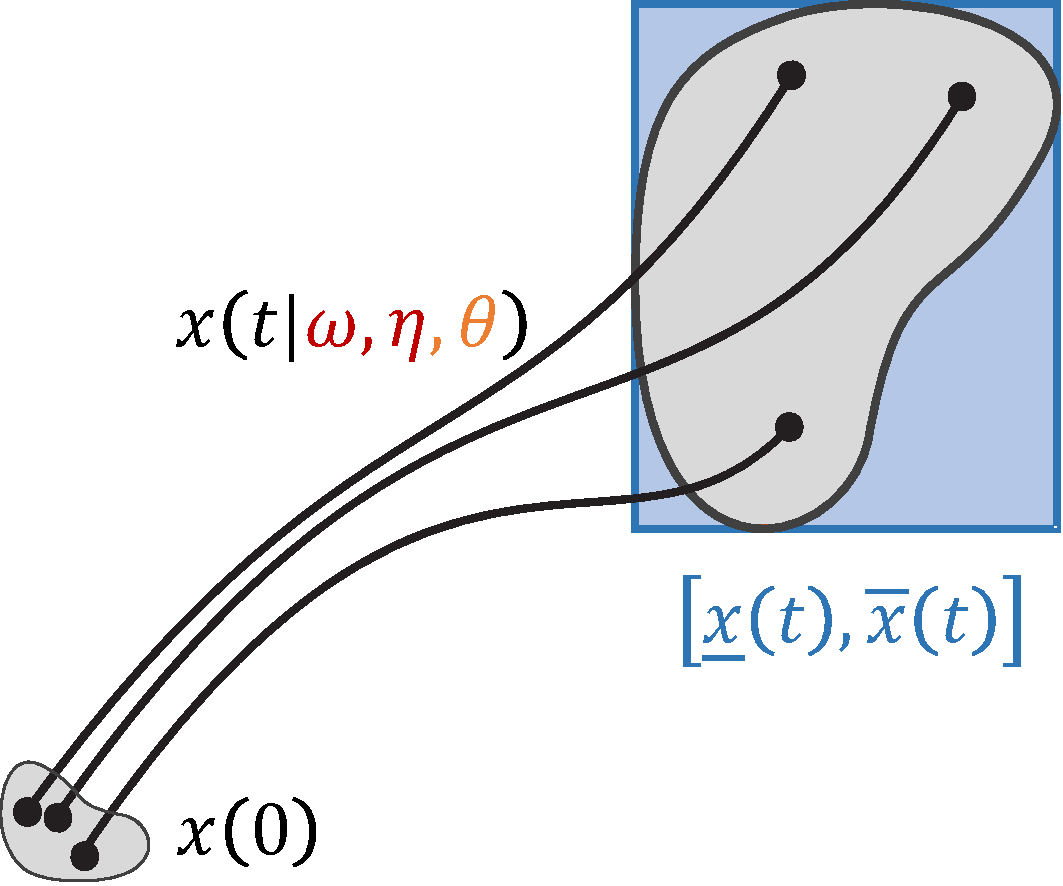
\includegraphics[width=0.35\linewidth]{img/interval-hull}
\end{center}
\begin{itemize}
	\item[\incarrow] To derive this predictor, two possible \alert{representations of the uncertainty} over $A(\theta)$ can be used.
\end{itemize}
\end{frame}

\begin{frame}{Step 2: Interval Uncertainty}
For all $\theta\in\hat{\Theta}(t)$,
{\orange$\quad\underline{A}\leq A(\theta)\leq\overline{A}
$}.
\begin{proposition}[Simple predictor of \cite{Efimov2012}]
{\small
\begin{align*}
{\blue \dot{\underline{x}}(s)} & = {\orange \underline{A}^{+}}\underline{x}^{+}(s)-{\orange\overline{A}^{+}}\underline{x}^{-}(s)-{\orange\underline{A}^{-}}\overline{x}^{+}(s)+{\orange\overline{A}^{-}}\overline{x}^{-}(s) +Bu(s)+\underline{\omega}(s),\\
{\blue \dot{\overline{x}}(s)} & = {\orange \overline{A}^{+}}\overline{x}^{+}(s)-{\orange\underline{A}^{+}}\overline{x}^{-}(s)-{\orange\overline{A}^{-}}\underline{x}^{+}(s)+{\orange\underline{A}^{-}}\underline{x}^{-}(s)
+Bu(s)+\overline{\omega}(s), \\
&  \underline{x}(t)=y_{1}(t)-\underline{\nu}_{1}(t),\;\overline{x}(t)=y_{1}(t)+\overline{\nu}_{1}(t), 
\end{align*}
}
ensures the inclusion property.
\end{proposition}
\begin{center}
	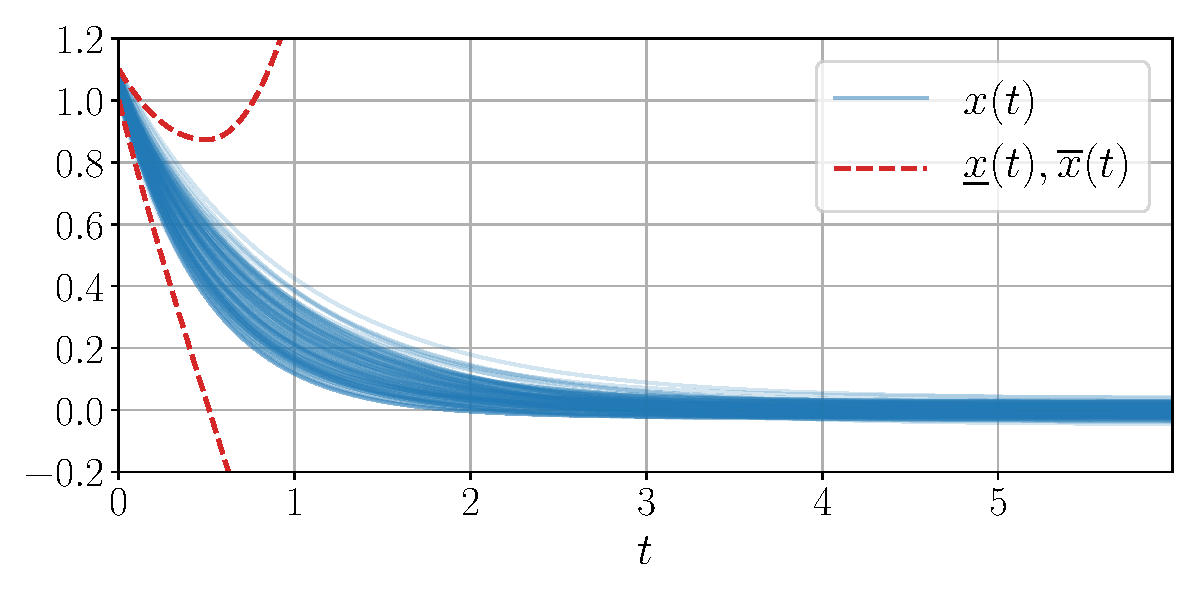
\includegraphics[width=0.6\linewidth]{img/observer}
	\vspace*{-1cm}
\end{center}
\end{frame}

\begin{frame}{Step 2: Polytopic Uncertainty} $\forall\theta\in\hat{\Theta}(t)$, ${\orange A(\theta)}\in\left\{ {\orange A_{0}+\sum_{i=1}^{2^{d}}\alpha_{i}\Delta A_{i}}:\alpha_{i}\geq0,\sum_{i=1}^{2^{d}}\alpha_{i}=1\right\}$
\begin{proposition}[Enhanced predictor of \cite{leurent2019interval}]
	{\small
	\begin{align*}
{\blue \dot{\underline{x}}(s)} & = {\orange A_{0}}\underline{x}(s)-{\orange \Delta A_{+}}\underline{x}^{-}(s)-{\orange \Delta A_{-}}\overline{x}^{+}(s)
+Bu(s)+\underline{\omega}(s) \\
{\blue \dot{\overline{x}}(s)} & = {\orange A_{0}}\overline{x}(s)+{\orange \Delta A_{+}}\overline{x}^{+}(s)+{\orange \Delta A_{-}}\underline{x}^{-}(s)\label{eq:interval-predictor}
+Bu(s)+\overline{\omega}(s) \\
& \underline{x}(t)=y_{1}(t)-\underline{\nu}_{1}(t),\;\overline{x}(t)=y_{1}(t)+\overline{\nu}_{1}(t),\nonumber 
	\end{align*}}
	ensures the inclusion property.
\end{proposition}
\begin{center}
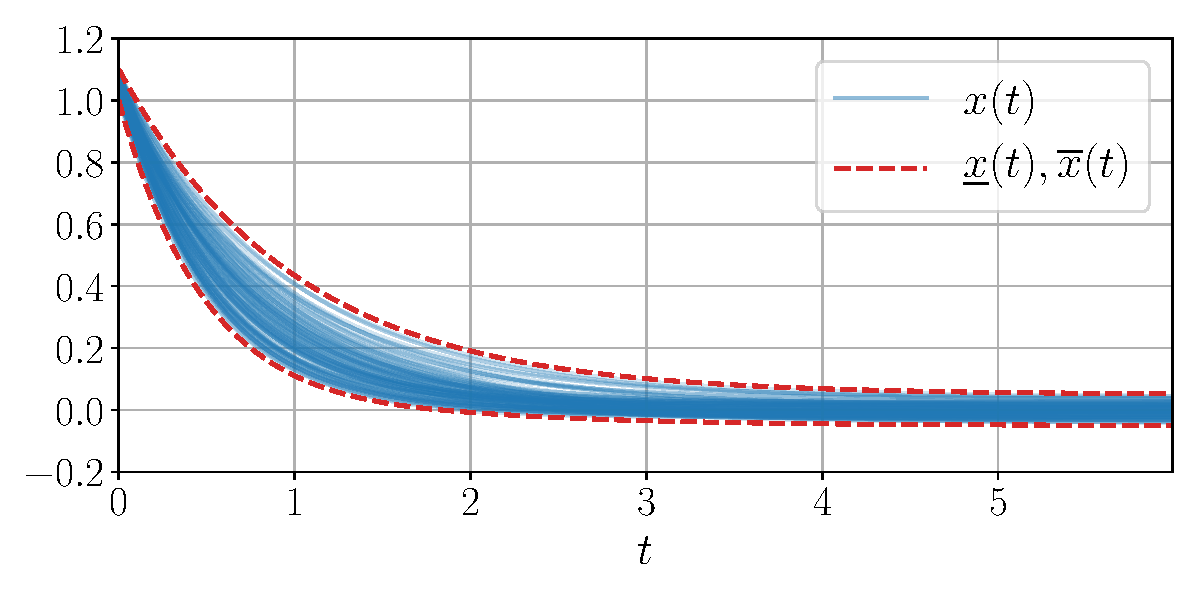
\includegraphics[width=0.6\linewidth]{img/predictor}
\vspace*{-1cm}
\end{center}
\end{frame}

\begin{frame}{Step 3: Robust Stabilization}
%Now that we have 
%$
%{\blue \ux(s)}\leq x(s)\leq{\blue \ox(s)},\quad\forall s\geq t,
%$

We want to \alert{stabilize} $$ {\blue \xi(t) = \begin{bmatrix}\underline{x}(t) \\ \overline{x}(t)\end{bmatrix}}$$


%
%Its dynamics can be written as \begin{equation}
%\dot{\xi}(t)=\cA_{0}\xi (t)+\cA_{1}\xi^{+}(t)+\cA_{2}\xi^{-}(t)+\cB u(t)+\delta(t),
%\end{equation}
%with $\delta(t)=\begin{bmatrix}
%\underline{\omega}(t) & \overline{\omega}(t)
%\end{bmatrix}^\top\in\Real^{2p}
%$
\begin{exampleblock}{Controller design}
We propose to look for a control in the form
\begin{equation*}
u(t)=K_{0}{\blue \xi(t)}+K_{1}{\blue \xi^{+}(t)}+K_{2}{\blue \xi^{-}(t)}+S{\red \begin{bmatrix}\underline{\omega}(t) & \overline{\omega}(t)\end{bmatrix}}^\top
\end{equation*}
\end{exampleblock}
\end{frame}

\begin{frame}{Step 3: Robust Stabilization}
Denote the closed-loop state matrices ${\green \cD_{i}}=\cA_{i}+\cB {\green K_{i}}$ for $i\in[3]$.

The gains $K_{0},K_{1},K_{2}$ have to respect the following restriction:
\begin{theorem}[ISS Stability]
	
	If there exist diagonal matrices $P$, $Q$, $Q_{+}$,
	$Q_{-}$, $Z_{+}$, $Z_{-}$, $\Psi_{+}$, $\Psi_{-}$, $\Psi$, $\Gamma\in\Real^{2p\times2p}$
	such that:
	\scriptsize
	\begin{gather*}
	{\green \Upsilon\preceq0},\;P+\min\{Z_{+},Z_{-}\}>0,\;\Gamma>0,\\
	Q+\min\{Q_{+},Q_{-}\}+2\min\{\Psi_{+},\Psi_{-}\}>0,
	\end{gather*}
	\vspace*{-0.8cm}\tiny \begin{gather*}
	\text{where }\quad {\green \Upsilon}=\left[\begin{array}{cccc}
	\Upsilon_{11} & \Upsilon_{12} & \Upsilon_{13} & P\\
	\Upsilon_{12}^{\top} & \Upsilon_{22} & \Upsilon_{23} & Z_{+}\\
	\Upsilon_{13}^{\top} & \Upsilon_{23}^{\top} & \Upsilon_{33} & -Z_{-}\\
	P & Z_{+} & -Z_{-} & -\Gamma
	\end{array}\right], \\
	\Upsilon_{11}=\cD_{0}^{\top}P+P\cD_{0}+Q,\;\Upsilon_{12}=\cD_{0}^{\top}Z_{+}+P\cD_{1}+\Psi_{+},\\
	\Upsilon_{13}=P\cD_{2}-\cD_{0}^{\top}Z_{-}-\Psi_{-},\;\Upsilon_{22}=Z_{+}\cD_{1}+\cD_{1}^{\top}Z_{+}+Q_{+},\\
	\Upsilon_{23}=Z_{+}\cD_{2}-\cD_{1}^{\top}Z_{-}+\Psi,\;\Upsilon_{33}=-Z_{-}\cD_{2}-\cD_{2}^{\top}Z_{-}+Q_{-},
	\end{gather*}
	\normalsize
	then ${\blue \xi(t)}$ is \alert{input-to-state stable} with respect
	to ${\red \underline{\omega},\overline{\omega}}$.
\end{theorem}
\end{frame}

\begin{frame}
\centering \LARGE Thank You!\\[1cm]
\large \emph{I am looking for a postdoctoral position.}
\end{frame}


\end{document}
